\section{Đánh giá tư thế ngủ sử dụng cảm biến gia tốc}
Tác giả tiến hành thử nghiệm bằng cách gắn bộ kit tại phần xương ức ở cổ khi ngủ. Phòng ngủ kín với nhiệt độ ổn định kín.  Đầu tiên, thiết bị sẽ được gắn lên vị trí đo bằng bang keo y tế. Khởi động thiết bị, sau đó tiến hành đăng nhập trên ứng dụng trên điện thoại. Cuối cùng kết nối với BLE với thiết bị phần cứng có tên là “Adafruit Playground” và chọn dịch vụ cảm biến gia tốc. Tác giả thử nghiệm theo từng tư thế ngủ bao gồm: nằm ngửa, nằm nghiêng trái, nằm sấp, nằm nghiêng phải. Mỗi tư thế sẽ được thử nghiệm trong 5 phút và cho ra kết quả tương đối chính xác. Khi chuyển các tư thế nằm ngủ, sẽ có 2 trường hợp xảy ra: 

\begin{itemize}
    \item Nếu chuyển động thay đổi tư thế nhẹ nhàng, kết quả vẫn có độ chính xác cao.
    
    \item Chuyển động nhanh có thể xảy ra và khó phát hiện đó là tư thế ngủ nào.
\end{itemize}

Trường hợp nằm ngủ với góc nghiêng (so với mặt phẳng ngang) lớn hơn 450, không được ghi nhận là tư thế ngủ. Tác giả xác nhận dữ liệu lấy ra từ cảm biến, dữ liệu truyền qua BLE, dữ liệu được lưu trữ trên đám mây đồng bộ với nhau, không có sự mất mát.

Các bước tiến hành thực nghiệm như Hình ~\ref{thucnghiem}:
\begin{itemize}
    \item Gắn cố định kit bằng băng ý tế lên phần xương ức ở cổ.
    
    \item Tiến hành đăng nhập.
    \item Lựa chọn thiết bị BLE.

    \item Kiểm tra kết quả

    \item Tiếp cận cơ bản mô hình học máy.
    
\end{itemize}
\begin{figure} [b!]
    \centering
    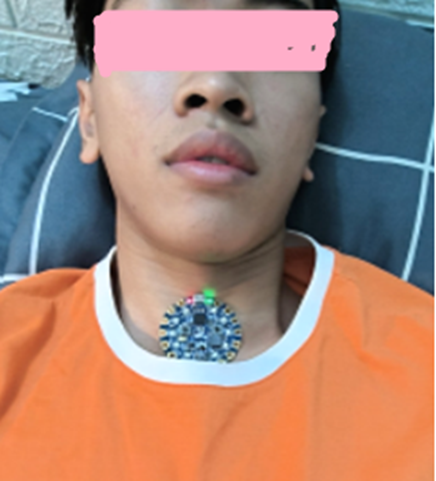
\includegraphics[width=0.6\linewidth]{images/thucnghiem.png}
    \caption{Thực nghiệm với kit Adafruit Playground}
    \label{thucnghiem}
\end{figure}


Một trong những nhiệm vụ mà tác giả được giao khi thực hiện khóa luận là phát triển một phần mềm ứng dụng cho phép người dùng sử dụng một cách đơn giản. Với nhận thức của tác giả, dựa trên góp ý của nhóm nghiên cứu, phần mềm ứng dụng phải đáp ứng những yêu cầu như dễ dàng thao tác, giao diện thân thiện, tính năng cơ bản.

Sau khi cài đặt, cửa sổ đăng nhập (cho người đã đăng ký) hoặc đăng ký mới có giao diện như trong Hình ~\ref{appAuth}. Với người mới bắt đầu sử dụng và muốn lưu trữ dữ liệu cần phải đăng ký tài khoản và xác thực qua email. Mục đích để xác định người đang sử dụng và lấy lại mật khẩu khi cần thiết.
\begin{figure} [h!]
    \centering
    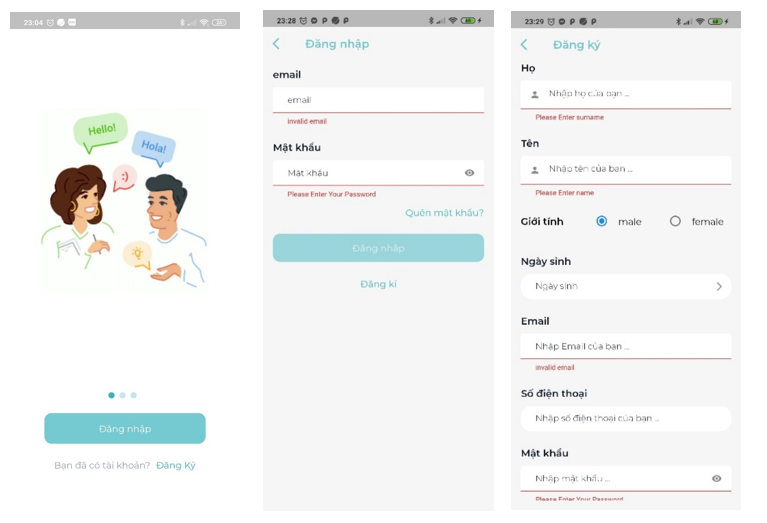
\includegraphics[width=0.8\linewidth]{images/appAuth.png}
    \caption{Các chức năng đăng ký, đăng nhập}
    \label{appAuth}
\end{figure}

\begin{figure}[h!]
    \centering
    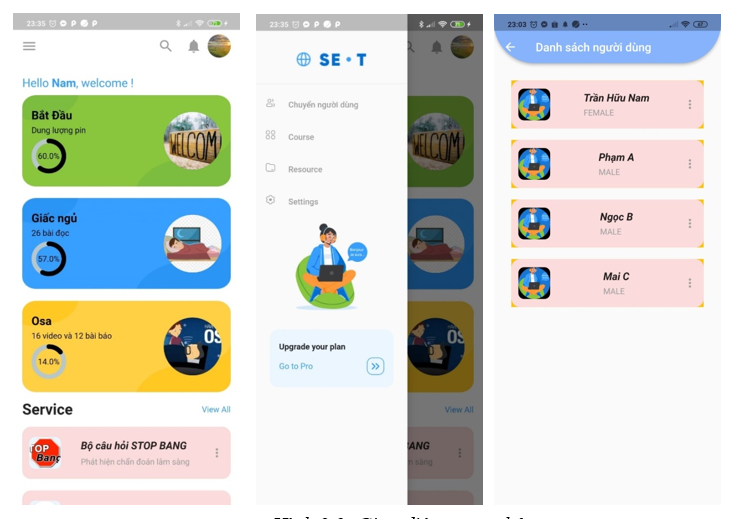
\includegraphics[width=0.8\linewidth]{images/app_cate.png}
    \caption{Giao diện trang chủ}
    \label{app_cate}
\end{figure}

Hình ~\ref{app_cate} là giao diện khi người dùng đăng nhập thành công, bao gồm các tính năng: Kết nối BLE và đọc dữ liệu, chuyển người dùng, xem thông tin người dùng v.v.


\begin{figure}
    \centering
    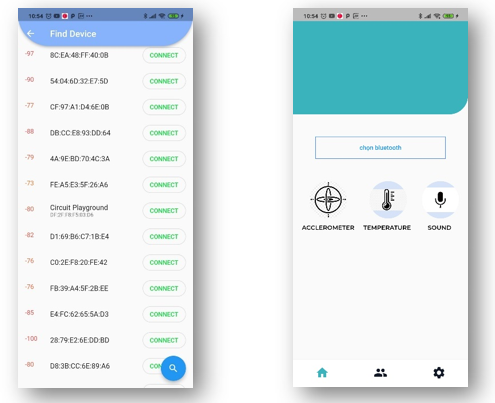
\includegraphics[width=0.8\linewidth]{images/app_ble.png}
    \caption{Kết nối với BLE và hiển thị dữ liệu}
    \label{app_ble}
\end{figure}

Hình ~\ref{app_ble} là giao diện kết thể hiện các thiết bị đang mở trạng thái quảng cáo. Sau khi chọn đúng thiết bị phần cứng thì giao diện sẽ chuyển tới màn hình chọn dịch vụ. Sau khi chọn dịch vụ cảm biến màn hình tự động chuyển đến màn hình hiển thị các biểu đồ. Trong khuôn khổ khoá luận, tác giả sử dụng so sánh ngưỡng dữ liệu thu được từ 3 trục của cảm biến gia tốc thu được với các giá trị đặt sẵn sau nhiều lần thực nghiệm Mã nguồn \ref{nguong}.

\begin{lstlisting}[float,language=C,caption=Tập lệnh đánh giá tư thế ngủ bằng ngưỡng, label=nguong,captionpos=b]
static Function getPositionSleep = (double x, double y, double z) {
    if ((-6.5 < y && y < 6.5)) {
      if (-7.07 < x && x < 7.07) {
        if (z > 0) {
          return 1; // ngua
        }
        if (z < 0) {
          return 4; //sap
        }
      }
      if (x > 3) return 2; //trai
      if (x < -3) return 3; //phai
  }
    return 6; // khong phai nam
  };

\end{lstlisting}



Hình ~\ref{appbieudo} là phần quan trọng nhất của ứng dụng. Phần đầu tiên là biểu đồ giá trị 3 trục theo thời gian thực. Phần 2 là tổng thời gian theo tư thế ngủ tính theo phút. Và cuối cùng là tư thế hiện tại của người dùng.
Tuy nhiên việc so sánh ngưỡng như vậy chưa mang tính thống kê trong khuôn khổ khoá luận. Vì vậy, các mô hình học máy cần phải được sử dụng trong tương lai để đánh giá và kết luận tư thế ngủ với độ chính xác cao. Theo đó, tư thế ngủ liên tục được cập nhật và tổng hợp sau mỗi 10 giây.

\begin{figure}
    \centering
    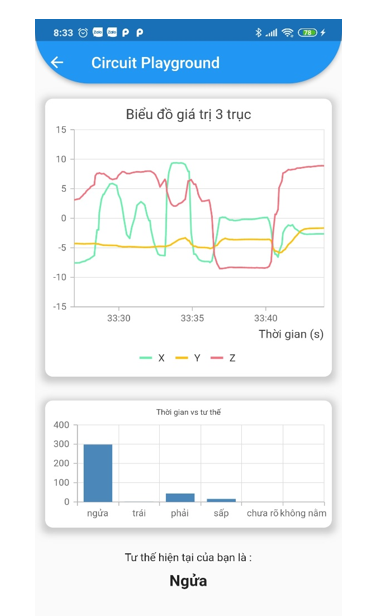
\includegraphics[width=0.75\linewidth]{images/appbieudo.png}
    \caption{Màn hình hiển thị giá trị của 3 trục cảm biến gia tốc}
    \label{appbieudo}
\end{figure}

\section{Học máy với dữ liệu đánh giá từ thiết bị}
Sau khi tìm hiểu những bước cơ bản từ chương 2 tác giả đã có những bước tiến hành như sau:

\begin{itemize}
    \item Thu thập dữ liệu và đánh nhãn: Tác giả thu tập 3859 mẫu dữ liệu theo từng tư thế ngủ: ngửa, nghiêng trái, nghiên phải và sấp với 1 đối tượng trong nhóm. Mỗi tư thế tác giả thực hiện trong 100 giây là dừng lại để đánh nhãn trực tiếp sau mỗi lần thử nghiệm. Việc lấy mẫu như vậy có tác dụng i) cân bằng dữ liệu ii)) tối ưu độ chính xác của nhãn.
    
    \item Phân tích dữ liệu: Xóa bỏ những dữ liệu ban đầu của mỗi hoạt động. Trích xuất tính năng theo miền thời gian (trung bình, phương sai, giá trị nhỏ nhất, giá trị lớn nhất,…) theo các của sổ 1 giây.
    \item Đánh giá tương quan và loại bỏ tính năng.

    \item Sử dụng các mô hình học máy.
    
\end{itemize}




\begin{figure} [!]
    \centering
    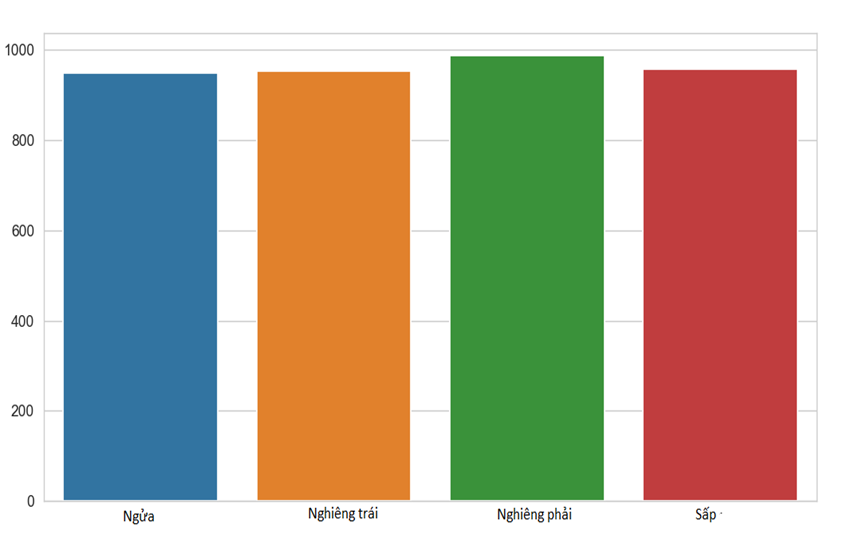
\includegraphics[width=0.75\linewidth]{images/hocmay_mau.png}
    \caption{Biểu đồ số lượng các mẫu}
    \label{hocmay_mau}
\end{figure}

Các thuật toán phân loại tiêu chuẩn khó có thể tối ưu được khi áp dụng trực tiếp cho dữ liệu chuỗi thời gian thô. Đầu tiên, tác giả chia dữ liệu thành các cửa sổ 3 giây. Sau đó, tác giả tạo các tính năng mới bằng cách tổng hợp 30 mẫu thô có trong mỗi phân đoạn 3 giây này.Để gán nhãn lớp cho các tính năng được chuyển đổi, tác giả sẽ lấy tư thế đa số trong của sổ đó. Ví dụ: tập dữ liệu thô có 100 hàng dữ liệu tuần tự.Vì vậy, sau khi tạo cửa sổ và tổng hợp (sử dụng kích thước cửa sổ = 30), nó sẽ được chuyển thành 10 hàng.
Có một điều nữa, tác giả lấy các cửa sổ chồng chéo với 50\% độ phủ. Điều này đảm bảo rằng mọi hàng tiếp theo trong tập dữ liệu được chuyển đổi cũng có một số thông tin từ dữ liệu trong cửa sổ trước đó.
Sau khi trích xuất tính năng, tác giả sẽ sử dụng ma trận tương quan Hình ~\ref{matrantuongquan} để đánh giá các tính năng.



\begin{figure}[!]
    \centering
    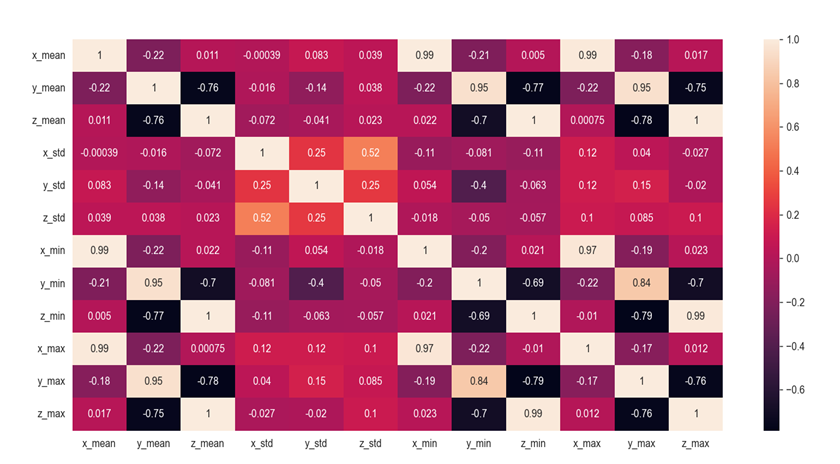
\includegraphics[width=1\linewidth]{images/matrantuongquan.png}
    \caption{Ma trận tương quan giữa các tính năng}
    \label{matrantuongquan}
\end{figure}

Tác giả sẽ loại bỏ đi những tính năng có hệ số tương quan > 0.95 để giảm thiểu thích thước dữ liệu.
Kết quả có độ chính xác lên tới 96\% trong việc đánh giá 4 tư thế ngủ từ tập kiểm tra chiếm 25\% dữ liệu thu thập bằng cách áp dụng mô hình SVM. Đây mới chỉ là những kết quả bước đầu với số lượng mẫu còn hạn chế và chỉ tập trung vào 4 tư thế cơ bản. Nếu chỉ so sánh việc phát hiện 4 tư thế thì độ chính xác thì kết quả của 2 phương pháp tương đương nhau. Tuy nhiên, nhược điểm của phương pháp đánh giá ngưỡng là khó phát hiện những chuyển động đột ngột, bất thường trong lúc ngủ mà hiện tại tác giả coi đây là những tư thế chưa xác định. Để giải quyết vấn đề này thì học máy được coi là phương pháp hiệu quả nhất. Tư thế nằm ngửa và nghiêng trái đang có sự nhầm lẫn có thể do bước loại bỏ các dữ liệu hoặc do bước đánh nhãn cho 1 cửa sổ Hình \ref{matrannhamlan}. 
\begin{figure} [!]
    \centering
    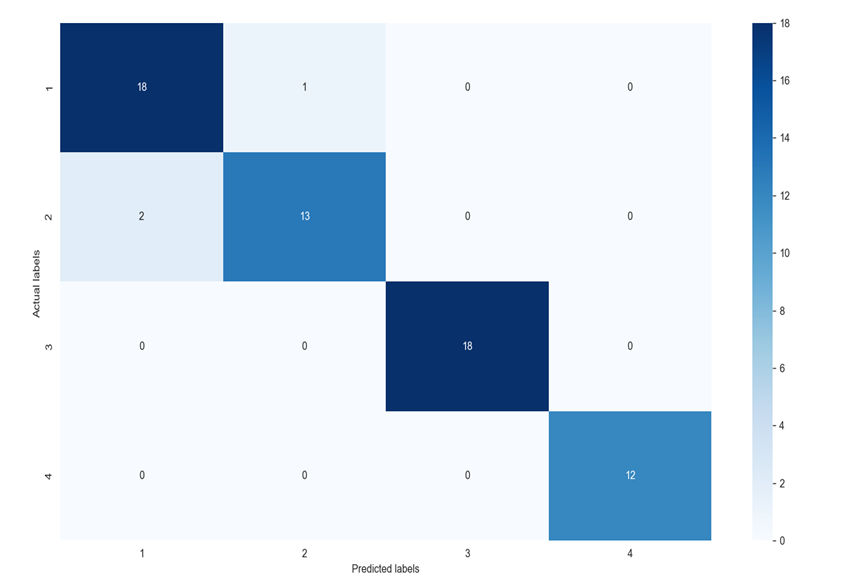
\includegraphics[width=1\linewidth]{images/matrannhamlan.png}
    \caption{Ma trận nhầm lẫn}
    \label{matrannhamlan}
\end{figure}